\documentclass[conference]{IEEEtran}
\IEEEoverridecommandlockouts
% The preceding line is only needed to identify funding in the first footnote. If that is unneeded, please comment it out.
\usepackage{cite}
\usepackage{amsmath,amssymb,amsfonts}
\usepackage{algorithmic}
\usepackage{graphicx}
\usepackage{textcomp}
\usepackage{xcolor}
\usepackage{booktabs}
\usepackage{csvsimple}
\usepackage{float}
\usepackage{caption}
\usepackage{tabularx}
\def\BibTeX{{\rm B\kern-.05em{\sc i\kern-.025em b}\kern-.08em
    T\kern-.1667em\lower.7ex\hbox{E}\kern-.125emX}}
\begin{document}

\title{Conference Paper Title*\\
{\footnotesize \textsuperscript{*}Note: Sub-titles are not captured in Xplore and
should not be used}
\thanks{Identify applicable funding agency here. If none, delete this.}
}

\author{\IEEEauthorblockN{1\textsuperscript{st} Given Name Surname}
\IEEEauthorblockA{\textit{dept. name of organization (of Aff.)} \\
\textit{name of organization (of Aff.)}\\
City, Country \\
email address or ORCID}
\and
\IEEEauthorblockN{2\textsuperscript{nd} Given Name Surname}
\IEEEauthorblockA{\textit{dept. name of organization (of Aff.)} \\
\textit{name of organization (of Aff.)}\\
City, Country \\
email address or ORCID}
\and
\IEEEauthorblockN{3\textsuperscript{rd} Given Name Surname}
\IEEEauthorblockA{\textit{dept. name of organization (of Aff.)} \\
\textit{name of organization (of Aff.)}\\
City, Country \\
email address or ORCID}
\and
\IEEEauthorblockN{4\textsuperscript{th} Given Name Surname}
\IEEEauthorblockA{\textit{dept. name of organization (of Aff.)} \\
\textit{name of organization (of Aff.)}\\
City, Country \\
email address or ORCID}
\and
\IEEEauthorblockN{5\textsuperscript{th} Given Name Surname}
\IEEEauthorblockA{\textit{dept. name of organization (of Aff.)} \\
\textit{name of organization (of Aff.)}\\
City, Country \\
email address or ORCID}
\and
\IEEEauthorblockN{6\textsuperscript{th} Given Name Surname}
\IEEEauthorblockA{\textit{dept. name of organization (of Aff.)} \\
\textit{name of organization (of Aff.)}\\
City, Country \\
email address or ORCID}
}

\maketitle

\begin{abstract}
% TODO
\end{abstract}

\begin{IEEEkeywords}
component, formatting, style, styling, insert
\end{IEEEkeywords}

\section{Introduction}

% TODO

\section{Pre-processing and description of datasets}

\subsection{Dataset 1: Apple Stock Data}

Pre-processing included converting the string date into a DateTime format. Converting strings to float and int datatypes, where appropriate. Renaming columns for convenience. The Closing\_Price column was a string type with a '\$' sign pre-pended to the front. This was removed and the feature was converted to a float value since the RNN requires all features to be numerical. The Year, Month, Day and Weekday features were extracted from the DateTime and converted into two dimensions using sine and cosine transformations. This was done because the RNN requires all features to be numerical. Volume, Open, High, Low, Date, Year, Month, Day, Weekday features were dropped since we are only interested in predicting the closing price for the day and some of the features were redundant. Here are the summary statistics before pre-processing:

\begin{table}[htbp]
	\caption{Summary statistics for Apple stock data}
	\resizebox{\columnwidth}{!}{
		\csvautobooktabular{../csv-descriptions/apple-raw-data-description.csv}
	}
	\label{tab:apple-stats}
\end{table}

The Apple stock data is non-stationary. The Apple stock data is a regression problem. The distributions were inspected using bar plots and no outliers or noise was found.

\subsection{Dataset 2: Cape Town weather data}

The data was sourced from Kaggle (https://www.kaggle.com/datasets/muthuj7/weather-dataset). For experimentation almost all features except the time and average temperature for the day was removed. Relevant features were extracted from the date (Year, Month, DayOfWeek, DayOfYear, WeekOfYear) and converted into two dimensions using sine and cosine transformations.

\begin{table}[htbp]
	\centering
	\caption{Summary statistics for Cape Town weather stock data}
	\scriptsize
	\scalebox{1.2}{
		\csvautobooktabular{../csv-descriptions/weather-stats.csv}
	}
	\label{tab:weather-stats}
\end{table}

The Cape Town weather data is non-stationary. The Cape Town weather data is a regression problem. The distributions were inspected and no outliers or noise was found.
 
\subsection{Dataset 3: Air quality data}

This data set was obtained from the UCI Machine Learning repository (https://archive.ics.uci.edu/dataset/360/air+quality), more information on the data set can be obtained there. For this experimentation, we will try and predict the PT08.S3(NOx) feature of the data set.

There were some empty rows and columns in the data set which were dropped. The HourOfDay, DayOfWeek and Month feature was extracted from the dates. The Year feature was not extracted as the data only spanned two years and the years did not provide any information. These features were converted to two dimensions using sine and cosine transformations. The ',' character was replaced with the '.' character in order to ensure that floats were correctly parsed. There were errors with the sensors where readings were less then or equal to 0, fill forward was used to replace these errors. PT08.S1(CO), C6H6(GT), PT08.S2(NMHC) were highly correlated with another feature so these features were dropped. The target feature also had these less or equal to 0 errors so all observations where the target feature had this error was dropped.

The Air quality data is stationary. The Air quality data is a regression problem. The distributions were inspected and no outliers or noise were found. These outliers were not reading/sensor errors but part of natural distribution of dataset.
\subsection{Dataset 4: }

\subsection{Dataset 5: }

\section{Background: Time series cross-validation}

\subsection{Time-series-split}

Creates folds where the observations of the validation set are always after the observations of the test set. The start of each fold is the beginning of the dataset. This allows for more splits, but creates leakage from future data to the model.

\subsection{Blocked cross-validation}

Works the same as time-series split but with added margins. One added between training and validation set. This is due to the correlation between observations at the end of the training set and beginning of validation set being very high, allowing the model to cheat a little bit. The second margin is added between the folds themselves, to prevent models from learning patterns from one fold iteration to the next. This allows for more splits and solves the data leakage issue but comes with the cost of increased computational requirements.

\section{Background: RNN network architectures}

This section covers current literature on the different RNN architectures experimented with in this paper.

\subsection{Elman and Jordan recurrent neural network}

Both the Elman and Jordan RNNs are three layer networks (input, hidden and output layer) with the Jordan RNN having an additional state vector (known as context units). The following notation is defined:

\begin{enumerate}
	\item $a,b,c,d,e,f,g \in \mathbb{Z}_{>0}$: A positive non-zero integer
	
	\item $x_t \in \mathbb{R}^a$: Input layer vector at time t
	\item $h_t \in \mathbb{R}^b$: Hidden layer vector at time t
	\item $y_t \in \mathbb{R}^c$: Output layer vector at time t
	
	\item $b_h \in \mathbb{R}^{d}$: Bias parameter vector for hidden layer
	\item $b_y \in \mathbb{R}^{e}$: Bias parameter vector for output layer
	
	\item $W_h \in \mathbb{R}^{d \times a}$: Input layer parameter matrix
	\item $U_h \in \mathbb{R}^{d \times b}$: Hidden layer parameter matrix
	
	\item $W_y \in \mathbb{R}^{e \times b}$: Output layer parameter matrix
	
	
	\item $\sigma_h: \mathbb{R}^e \to \mathbb{R}^b $: Activation function for hidden layer
	\item $\sigma_y: \mathbb{R}^e \to \mathbb{R}^c $: Activation function for output layer
\end{enumerate}

% https://spotintelligence.com/2023/02/01/elman-rnn/

% https://en.wikipedia.org/wiki/Recurrent_neural_network

The Elman RNN hidden state $h_t$ depends on both the input vector $x_t$ and the previous hidden state $h_t$ (this is the context vector). At each time the following is computed:

\begin{enumerate}
	\item $h_t = \sigma_h(W_h x_t + U_h h_{t-1} + b_h)$: 
	\item $y_t = \sigma_y(W_y h_t + b_y)$: 
\end{enumerate}

This is known as the forward pass. Some specified learning rule is applied in order to adjust the parameters of the model. For example we could calculate gradients of parameters with respect to loss and back-propagate in a backward pass. The previous hidden state $h_t$ is brought forward to next iteration.

The following additional components are added to the Jordan RNN:

\begin{enumerate}
	\item $s_t \in \mathbb{R}^f$: State layer vector at time t
	
	\item $b_s \in \mathbb{R}^{g}$: Bias parameter vector for state layer
	
	\item $W_{s,s} \in \mathbb{R}^{g \times f}$: State parameter matrix
	\item $W_{s,y} \in \mathbb{R}^{g \times c}$: State parameter matrix
	
	\item $\sigma_s: \mathbb{R}^g \to \mathbb{R}^f$: Activation function for state layer
	
	
	
\end{enumerate}

With the following updates at each time step:

\begin{enumerate}
	\item $h_t = \sigma_h(W_h x_t + U_h s_t + b_h)$: 
	\item $y_t = \sigma_y(W_y h_t + b_y)$: 
	\item $s_t = \sigma_s(W_{s,s} s_{t-1} + W_{s,y} y_{t-1} + b_s)$: 
\end{enumerate}

As we can see the hidden layer $h_t$ in a Jordan RNN is updated using a state layer vector $s_t$ (context units) instead of the previous hidden layer $h_{t-1}$. The state layer vector is updated using the previous state $s_{t-1}$ and the previous output $y_{t-1}$. Both models were implemented using the \texttt{torch} package exactly as described here.


\subsection{Multi-recurrent neural network}

For brevity the absolute dimensions of matrices and vectors are not specified but can be implied.

\subsubsection{Memory architecture and configuration}

Layer link ratio determines what proportion of the new layer activations are stored. Self link ratios determine what proportion of the previous memory is retained. Ratios between links determine if we have sluggish state-based memory bank. rapid memory bank or stable memory bank.

Memory composition is a hyper parameter which is specified as positive integers $i$, $h$, $o$ where $i$ is the allocation for input, $h$ is allocation for hidden and $o$ is allocation for output.

It is an extension of the state from an Elman or Jordan RNN which is keeps information from potentially all layers and is more dynamic as we can specify ratios.

Based off the memory composition we calculate the following:

\begin{enumerate}
	\item $n_M$: allocated number of memory banks for type $M$ which would be input, hidden, output.
	\item $\frac{i}{n_M}$: layer-link ratio for $i=n_m, \dots, 2, 1$
	\item $1 - \frac{i}{n_M}$: self-link ratio for $i=n_m, \dots, 2, 1$
\end{enumerate}





\subsubsection{Forward pass}

Inputs and memory banks fed to input layer, input layer outputs fed into hidden layer, hidden layer outputs and biases fed to output layer to produce network output.

Output layer outputs and current memory bank are copied using using layer link ratio and self link ratios.

Memory bank is updated. Weights and biases are updated using back-propagation.

\begin{enumerate}
	\item $n_i$: allocated number of memory banks for input
	\item $n_o$: allocated number of memory banks for output
	\item $n_h$: allocated number of memory banks for hidden
	\item $I_{t-1}$: input layer outputs at time $t-1$
	\item $H_{t-1}$: hidden layer outputs at time $t-1$
	\item $O_{t-1}$: output layer outputs at time $t-1$
	\item $W_{i_h}$: weights from input layer to hidden layer
	\item $W_{i_o}$: weights from hidden layer to output layer
	\item $W_{M_{ih}}$: weights of input memory bank to hidden layer
	\item $W_{M_{hh}}$: weights of hidden memory bank to hidden layer
	\item $W_{M_{oh}}$: weights of output memory bank to hidden layer
	\item $M_{ih}$: input memory bank to hidden layer
	\item $M_{hh}$: hidden memory bank to hidden layer
	\item $M_{oh}$: output memory bank to hidden layer
	\item $f$: activation function
	\item $b_i$: input layer biases
	\item $b_h$: hidden layer biases
\end{enumerate}

Updates to memory during forward pass:

\begin{enumerate}[]
	\item $M_{t_{i}} = \left(\tfrac{1}{n_{i}} \times I_{t-1}\right) + \left(1 - \tfrac{1}{n_{i}}\right) \times M_{t-1_{i}}$
	
	\item $M_{t_{h}} = \left(\tfrac{1}{n_{h}} \times H_{t-1}\right) + \left(1 - \tfrac{1}{n_{h}}\right) \times M_{t-1_{h}}$
	
	\item $M_{t_{o}} = \left(\tfrac{1}{n_{o}} \times O_{t-1}\right) + \left(1 - \tfrac{1}{n_{o}}\right) \times M_{t-1_{o}}$
\end{enumerate}

Outputs of hidden layer at time $t$ are:
\begin{align*}
	H_{t} &= f\Big( \sum W_{ih} I_{t} + \sum W_{Mi h} M_{t_i} \notag \\
	&\quad + \sum W_{Mh h} M_{t_h} + \sum W_{Mo h} M_{t_o} + b_{i} \Big)
\end{align*}

Outputs for output layer at time $t$ is: $O_{t} = \sum W_{h_o} H_{t} + b_{h}$








\section{Implementation}

The models were implemented using \texttt{torch} modules using the exact mathematical definitions defined in the background section. Dropout and early stopping was added to prevent deter over-fitting. $tanh$ actiavtion functions were used for consistency across models.


% Selected optimization algorithms and loss functions
% How under-fitting and over-fitting was prevented
% Settings for hyper-parameters
% Neural network architecture
% Performance measures
% Best simple RNN was chosen

\section{Empirical process}

Data was preprocessed into required format. This means recognising and dealing with noisy data, outliers, class imbalances and so forth. The models were tested with a base line model. If models began over-fitting too much, the weight decay and dropout was increased. The learning rate would be decreased if oscillation around the local minima began. The momentum parameter of the Adam optimizer was modified if the convergence seemed slow. The data was split was 70\% training and 30\% test. The training data was used in cross-validation. The distribution of features over time was plotted in order to better understand the features.

\section{Results \& discussion}

Scaling is necessary for data in an RNN. Scalers was trained on each training fold which did not include the test data. This ensures no data leakage.

\subsubsection{Dataset 1: Apple Stock Data}

Here are the parameter choices for the Elman model:

\begin{enumerate}[]
	\item Cross validation of 8 folds was used, due to small size of data set.
	\item A robust scaler was used.
	\item Dropout of 0.1 was used.
	\item A batch size of 128 was used.
	\item Learning rate of 0.005, increased from 0.001 after noticing slow convergence.
	\item A weight decay of 0.0001 which was increased from default of 0 due to detected over-fitting
	\item A early stopping patience of 20 which was increased from 10 originally after it was noticed that the algorithm was finding better local minima if given the opportunity.
	\item Model trained for 150 epochs in an attempt to find minima.
\end{enumerate}

The Jordan model uses the same parameters with a state layer size of 32.

Here is the distribution of the stock data:

\begin{figure}[H] 
	\centering
	\includegraphics[width=1.0\linewidth]{../images/apple-closing-price-over-time.pdf}
	\caption{Apple closing price over time}
	\label{fig:apple-closing}
\end{figure}

We can see it is very stochastic. There is also very little data. This data set will mainly showcase the shortcomings of the RNNs with small datasets. 

The hidden layer size of 32 seemed to under-fit the data. There is simply not enough data to for the Elman model to learn. Here we can see this with the predictions:

\begin{figure}[H] 
	\centering
	\includegraphics[width=1.0\linewidth]{../images/apple-elman-h32-actual-vs-predicted.pdf}
	\caption{Apple closing price over time predictions (Elman hidden year size 32)}
	\label{fig:apple-closing-predictions}
\end{figure}

The Jordan model appears to do well in the test folds until it reaches the fold with a massive price increase where performance dwindles.

\begin{figure}[H] 
	\centering
	\includegraphics[width=1.0\linewidth]{../images/apple-jordan-h32-actual-vs-predicted.pdf}
	\caption{Apple closing price over time predictions (Jordan hidden layer size 32)}
	\label{fig:apple-closing-predictions-jordan}
\end{figure}

\begin{table}[htbp]
	\caption{Absolute difference between prediction and actual for best fold model (for unseen Apple stock data)}
	\resizebox{\columnwidth}{!}{
		\csvautobooktabular{../csv-descriptions/apple-rnn-results.csv}
	}
	\label{tab:apple-rnn-summary}
\end{table}



\subsubsection{Dataset 2: Cape Town Weather Data}

Here are the Elman RNN parameter choices for this dataset:

\begin{enumerate}[]
	\item Cross validation of 6 folds was used, due to size of data set and computational restrictions.
	\item A robust scaler was used.
	\item Dropout of 0.2 was used.
	\item A batch size of 128 was used.
	\item Learning rate of 0.002, increased from 0.001 after noticing slow convergence.
	\item A weight decay of 0.0001 which was increased from default of 0 due to detected over-fitting
	\item A early stopping patience of 20 which was increased from 10 originally after it was noticed that the algorithm was finding better local minima if given the opportunity.
	\item Model trained for 100 epochs.
\end{enumerate}

The same parameters were used then for the Jordan RNN with a state layer size of 32, with no issues arising.

The following is the distribution of the weather data for Cape Town over time:

\begin{figure}[htbp] 
	\centering
	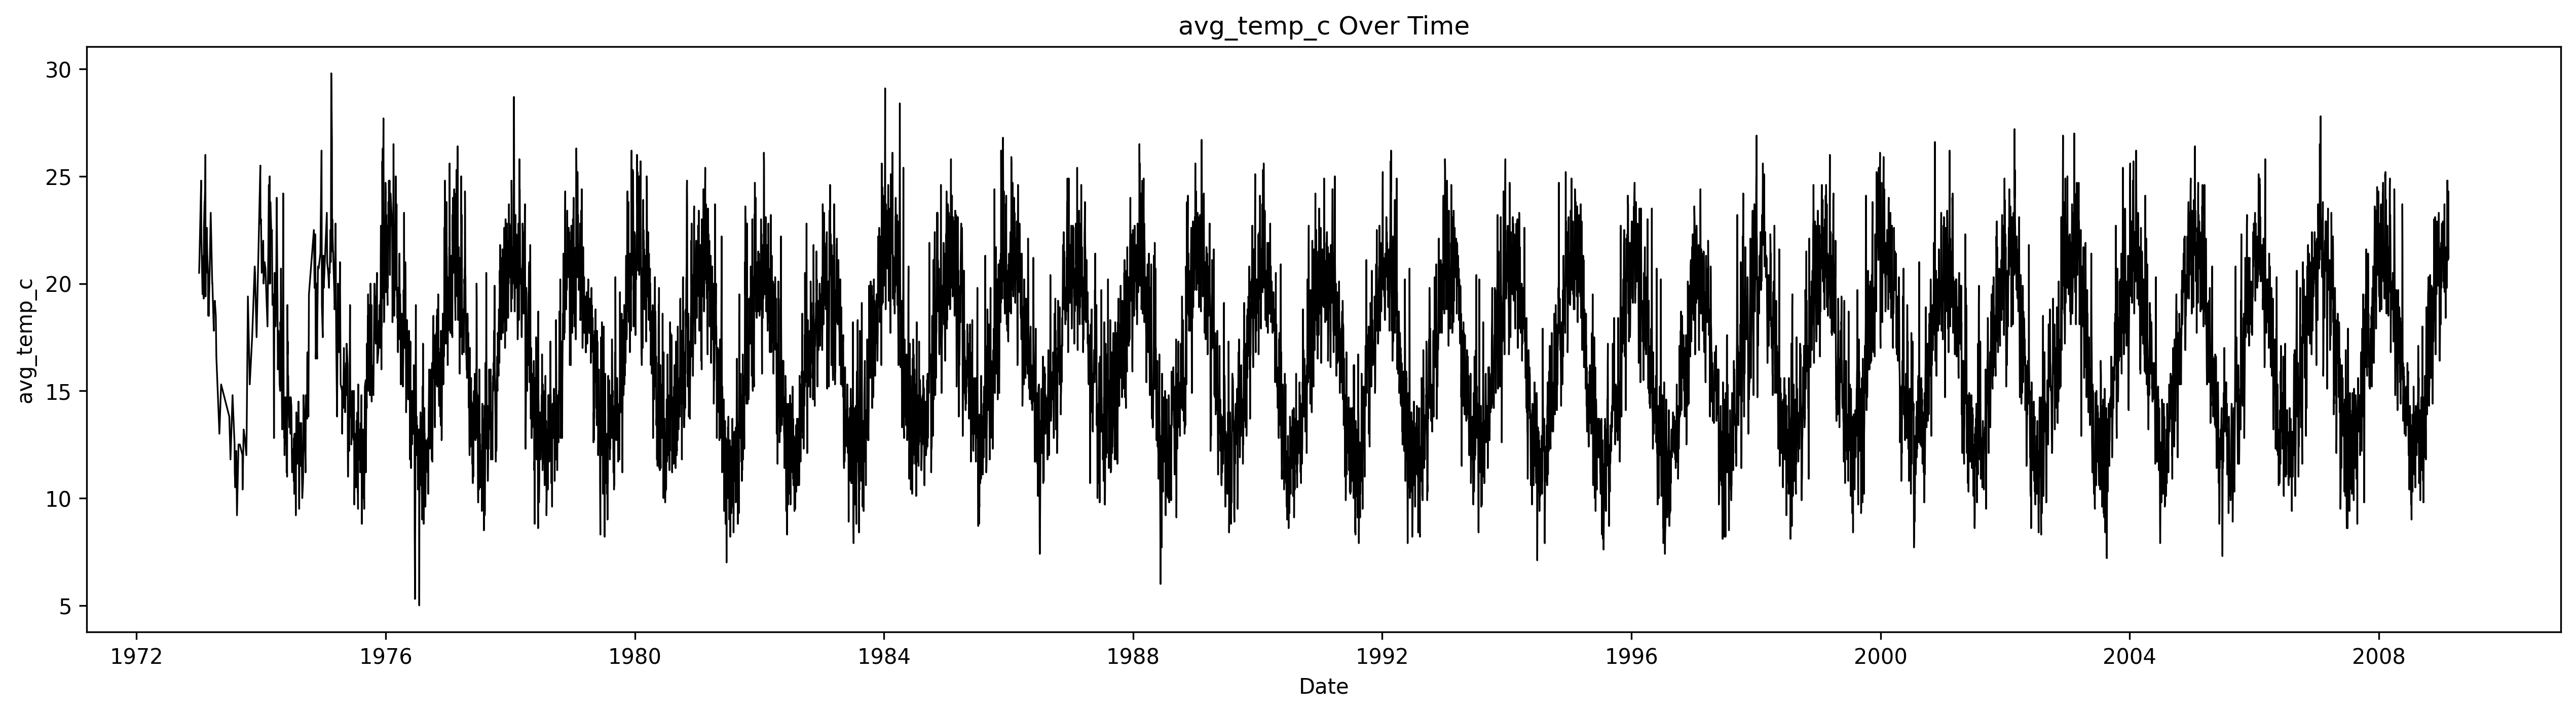
\includegraphics[width=1.0\linewidth]{../images/weather-over-time.pdf}
	\caption{Cape Town weather over time}
	\label{fig:cape-town-weather-time}
\end{figure}

The extreme cyclic nature made it very possible that the model would over-fit. The model did over-fit but surprisingly the validation performance was better then the test performance. Altering the learning rate, weight decay or dropout did not alter this. The performance is relatively good considering it only uses one raw feature. If the previous day's weather was included as a feature this would probably greatly increase the performance. Other external data would also greatly increase the performance. Here are the results from the cross-validation:

\begin{table}[htbp]
	\caption{Absolute difference between prediction and actual for best fold model (for unseen Cape Town weather data)}
	\resizebox{\columnwidth}{!}{
		\csvautobooktabular{../csv-descriptions/weather-rnn-results.csv}
	}
	\label{tab:weather-rnn-summary}
\end{table}

\begin{figure}[H] 
	\centering
	\includegraphics[width=1.0\linewidth]{../images/weather-elman-h32-actual-vs-predicted.pdf}
	\caption{Weather over time predictions (Jordan hidden layer size 32)}
	\label{fig:weather-predictions-elman}
\end{figure}

\subsubsection{Dataset 3: Air quality dataset}

\begin{table}[htbp]
	\caption{Absolute difference between prediction and actual for best fold model (for unseen Air quality data)}
	\resizebox{\columnwidth}{!}{
		\csvautobooktabular{../csv-descriptions/airquality-rnn-results.csv}
	}
	\label{tab:weather-rnn-summary}
\end{table}

\section{Conclusion}

\section{Ease of Use}

\subsection{Maintaining the Integrity of the Specifications}

The IEEEtran class file is used to format your paper and style the text. All margins, 
column widths, line spaces, and text fonts are prescribed; please do not 
alter them. You may note peculiarities. For example, the head margin
measures proportionately more than is customary. This measurement 
and others are deliberate, using specifications that anticipate your paper 
as one part of the entire proceedings, and not as an independent document. 
Please do not revise any of the current designations.

\section{Prepare Your Paper Before Styling}
Before you begin to format your paper, first write and save the content as a 
separate text file. Complete all content and organizational editing before 
formatting. Please note sections \ref{AA}--\ref{SCM} below for more information on 
proofreading, spelling and grammar.

Keep your text and graphic files separate until after the text has been 
formatted and styled. Do not number text heads---{\LaTeX} will do that 
for you.

\subsection{Abbreviations and Acronyms}\label{AA}
Define abbreviations and acronyms the first time they are used in the text, 
even after they have been defined in the abstract. Abbreviations such as 
IEEE, SI, MKS, CGS, ac, dc, and rms do not have to be defined. Do not use 
abbreviations in the title or heads unless they are unavoidable.

\subsection{Units}
\begin{itemize}
\item Use either SI (MKS) or CGS as primary units. (SI units are encouraged.) English units may be used as secondary units (in parentheses). An exception would be the use of English units as identifiers in trade, such as ``3.5-inch disk drive''.
\item Avoid combining SI and CGS units, such as current in amperes and magnetic field in oersteds. This often leads to confusion because equations do not balance dimensionally. If you must use mixed units, clearly state the units for each quantity that you use in an equation.
\item Do not mix complete spellings and abbreviations of units: ``Wb/m\textsuperscript{2}'' or ``webers per square meter'', not ``webers/m\textsuperscript{2}''. Spell out units when they appear in text: ``. . . a few henries'', not ``. . . a few H''.
\item Use a zero before decimal points: ``0.25'', not ``.25''. Use ``cm\textsuperscript{3}'', not ``cc''.)
\end{itemize}

\subsection{Equations}
Number equations consecutively. To make your 
equations more compact, you may use the solidus (~/~), the exp function, or 
appropriate exponents. Italicize Roman symbols for quantities and variables, 
but not Greek symbols. Use a long dash rather than a hyphen for a minus 
sign. Punctuate equations with commas or periods when they are part of a 
sentence, as in:
\begin{equation}
a+b=\gamma\label{eq}
\end{equation}

Be sure that the 
symbols in your equation have been defined before or immediately following 
the equation. Use ``\eqref{eq}'', not ``Eq.~\eqref{eq}'' or ``equation \eqref{eq}'', except at 
the beginning of a sentence: ``Equation \eqref{eq} is . . .''

\subsection{\LaTeX-Specific Advice}

Please use ``soft'' (e.g., \verb|\eqref{Eq}|) cross references instead
of ``hard'' references (e.g., \verb|(1)|). That will make it possible
to combine sections, add equations, or change the order of figures or
citations without having to go through the file line by line.

Please don't use the \verb|{eqnarray}| equation environment. Use
\verb|{align}| or \verb|{IEEEeqnarray}| instead. The \verb|{eqnarray}|
environment leaves unsightly spaces around relation symbols.

Please note that the \verb|{subequations}| environment in {\LaTeX}
will increment the main equation counter even when there are no
equation numbers displayed. If you forget that, you might write an
article in which the equation numbers skip from (17) to (20), causing
the copy editors to wonder if you've discovered a new method of
counting.

{\BibTeX} does not work by magic. It doesn't get the bibliographic
data from thin air but from .bib files. If you use {\BibTeX} to produce a
bibliography you must send the .bib files. 

{\LaTeX} can't read your mind. If you assign the same label to a
subsubsection and a table, you might find that Table I has been cross
referenced as Table IV-B3. 

{\LaTeX} does not have precognitive abilities. If you put a
\verb|\label| command before the command that updates the counter it's
supposed to be using, the label will pick up the last counter to be
cross referenced instead. In particular, a \verb|\label| command
should not go before the caption of a figure or a table.

Do not use \verb|\nonumber| inside the \verb|{array}| environment. It
will not stop equation numbers inside \verb|{array}| (there won't be
any anyway) and it might stop a wanted equation number in the
surrounding equation.

\subsection{Some Common Mistakes}\label{SCM}
\begin{itemize}
\item The word ``data'' is plural, not singular.
\item The subscript for the permeability of vacuum $\mu_{0}$, and other common scientific constants, is zero with subscript formatting, not a lowercase letter ``o''.
\item In American English, commas, semicolons, periods, question and exclamation marks are located within quotation marks only when a complete thought or name is cited, such as a title or full quotation. When quotation marks are used, instead of a bold or italic typeface, to highlight a word or phrase, punctuation should appear outside of the quotation marks. A parenthetical phrase or statement at the end of a sentence is punctuated outside of the closing parenthesis (like this). (A parenthetical sentence is punctuated within the parentheses.)
\item A graph within a graph is an ``inset'', not an ``insert''. The word alternatively is preferred to the word ``alternately'' (unless you really mean something that alternates).
\item Do not use the word ``essentially'' to mean ``approximately'' or ``effectively''.
\item In your paper title, if the words ``that uses'' can accurately replace the word ``using'', capitalize the ``u''; if not, keep using lower-cased.
\item Be aware of the different meanings of the homophones ``affect'' and ``effect'', ``complement'' and ``compliment'', ``discreet'' and ``discrete'', ``principal'' and ``principle''.
\item Do not confuse ``imply'' and ``infer''.
\item The prefix ``non'' is not a word; it should be joined to the word it modifies, usually without a hyphen.
\item There is no period after the ``et'' in the Latin abbreviation ``et al.''.
\item The abbreviation ``i.e.'' means ``that is'', and the abbreviation ``e.g.'' means ``for example''.
\end{itemize}
An excellent style manual for science writers is \cite{b7}.

\subsection{Authors and Affiliations}
\textbf{The class file is designed for, but not limited to, six authors.} A 
minimum of one author is required for all conference articles. Author names 
should be listed starting from left to right and then moving down to the 
next line. This is the author sequence that will be used in future citations 
and by indexing services. Names should not be listed in columns nor group by 
affiliation. Please keep your affiliations as succinct as possible (for 
example, do not differentiate among departments of the same organization).

\subsection{Identify the Headings}
Headings, or heads, are organizational devices that guide the reader through 
your paper. There are two types: component heads and text heads.

Component heads identify the different components of your paper and are not 
topically subordinate to each other. Examples include Acknowledgments and 
References and, for these, the correct style to use is ``Heading 5''. Use 
``figure caption'' for your Figure captions, and ``table head'' for your 
table title. Run-in heads, such as ``Abstract'', will require you to apply a 
style (in this case, italic) in addition to the style provided by the drop 
down menu to differentiate the head from the text.

Text heads organize the topics on a relational, hierarchical basis. For 
example, the paper title is the primary text head because all subsequent 
material relates and elaborates on this one topic. If there are two or more 
sub-topics, the next level head (uppercase Roman numerals) should be used 
and, conversely, if there are not at least two sub-topics, then no subheads 
should be introduced.

\subsection{Figures and Tables}
\paragraph{Positioning Figures and Tables} Place figures and tables at the top and 
bottom of columns. Avoid placing them in the middle of columns. Large 
figures and tables may span across both columns. Figure captions should be 
below the figures; table heads should appear above the tables. Insert 
figures and tables after they are cited in the text. Use the abbreviation 
``Fig.~\ref{fig}'', even at the beginning of a sentence.

\begin{table}[htbp]
\caption{Table Type Styles}
\begin{center}
\begin{tabular}{|c|c|c|c|}
\hline
\textbf{Table}&\multicolumn{3}{|c|}{\textbf{Table Column Head}} \\
\cline{2-4} 
\textbf{Head} & \textbf{\textit{Table column subhead}}& \textbf{\textit{Subhead}}& \textbf{\textit{Subhead}} \\
\hline
copy& More table copy$^{\mathrm{a}}$& &  \\
\hline
\multicolumn{4}{l}{$^{\mathrm{a}}$Sample of a Table footnote.}
\end{tabular}
\label{tab1}
\end{center}
\end{table}

\begin{figure}[htbp]
%\centerline{\includegraphics{fig1.png}}
\caption{Example of a figure caption.}
\label{fig}
\end{figure}

Figure Labels: Use 8 point Times New Roman for Figure labels. Use words 
rather than symbols or abbreviations when writing Figure axis labels to 
avoid confusing the reader. As an example, write the quantity 
``Magnetization'', or ``Magnetization, M'', not just ``M''. If including 
units in the label, present them within parentheses. Do not label axes only 
with units. In the example, write ``Magnetization (A/m)'' or ``Magnetization 
\{A[m(1)]\}'', not just ``A/m''. Do not label axes with a ratio of 
quantities and units. For example, write ``Temperature (K)'', not 
``Temperature/K''.

\section*{Acknowledgment}

The preferred spelling of the word ``acknowledgment'' in America is without 
an ``e'' after the ``g''. Avoid the stilted expression ``one of us (R. B. 
G.) thanks $\ldots$''. Instead, try ``R. B. G. thanks$\ldots$''. Put sponsor 
acknowledgments in the unnumbered footnote on the first page.

\section*{References}

Please number citations consecutively within brackets \cite{b1}. The 
sentence punctuation follows the bracket \cite{b2}. Refer simply to the reference 
number, as in \cite{b3}---do not use ``Ref. \cite{b3}'' or ``reference \cite{b3}'' except at 
the beginning of a sentence: ``Reference \cite{b3} was the first $\ldots$''

Number footnotes separately in superscripts. Place the actual footnote at 
the bottom of the column in which it was cited. Do not put footnotes in the 
abstract or reference list. Use letters for table footnotes.

Unless there are six authors or more give all authors' names; do not use 
``et al.''. Papers that have not been published, even if they have been 
submitted for publication, should be cited as ``unpublished'' \cite{b4}. Papers 
that have been accepted for publication should be cited as ``in press'' \cite{b5}. 
Capitalize only the first word in a paper title, except for proper nouns and 
element symbols.

For papers published in translation journals, please give the English 
citation first, followed by the original foreign-language citation \cite{b6}.

\begin{thebibliography}{00}
\bibitem{b1} G. Eason, B. Noble, and I. N. Sneddon, ``On certain integrals of Lipschitz-Hankel type involving products of Bessel functions,'' Phil. Trans. Roy. Soc. London, vol. A247, pp. 529--551, April 1955.
\bibitem{b2} J. Clerk Maxwell, A Treatise on Electricity and Magnetism, 3rd ed., vol. 2. Oxford: Clarendon, 1892, pp.68--73.
\bibitem{b3} I. S. Jacobs and C. P. Bean, ``Fine particles, thin films and exchange anisotropy,'' in Magnetism, vol. III, G. T. Rado and H. Suhl, Eds. New York: Academic, 1963, pp. 271--350.
\bibitem{b4} K. Elissa, ``Title of paper if known,'' unpublished.
\bibitem{b5} R. Nicole, ``Title of paper with only first word capitalized,'' J. Name Stand. Abbrev., in press.
\bibitem{b6} Y. Yorozu, M. Hirano, K. Oka, and Y. Tagawa, ``Electron spectroscopy studies on magneto-optical media and plastic substrate interface,'' IEEE Transl. J. Magn. Japan, vol. 2, pp. 740--741, August 1987 [Digests 9th Annual Conf. Magnetics Japan, p. 301, 1982].
\bibitem{b7} M. Young, The Technical Writer's Handbook. Mill Valley, CA: University Science, 1989.
\end{thebibliography}
\vspace{12pt}
\color{red}
IEEE conference templates contain guidance text for composing and formatting conference papers. Please ensure that all template text is removed from your conference paper prior to submission to the conference. Failure to remove the template text from your paper may result in your paper not being published.

\end{document}
